\chapter{PCB Security basics}
A Printed Circuit Board(PCB) are objects that connect electronic, or not, devices together.
They are usually characterized by:
\begin{itemize}
  \item a non conductive support, that is usually 
  \item a mechanical robustness, meaning that is sturdy to mechanical modification(eg. bending)
  \item can connect electronical components
\end{itemize}
\begin{section}{PCB types}
  There are 3 main types of PCBs:
  \begin{itemize}
    \item Single sided PCBs, the simplest kind. It has one side to put components on and the other
      one for routing them.
    \item Double sided PCBs, in which components can be placed and routed on both sides, being more
      flexible than the single sided ones.
    \item Multi-layer PCBs, in which there are multiple layers in which the components can be placed
      and routed. They are the most complex and expensive kind of PCBs, but allows to partially
      ignore the space constraints of the other two kinds.
  \end{itemize}
\end{section}

\begin{section}{Materials and packages}
  Lets now talk for a second about what a PCB is made of. First of all, it has an insulating layer,
  usually made up of glass, with the Flame Retardant 4(FR4) being the most common. The metalization
  layer is usually made up of copper, and the components, which usually were through-hole, are now
  surface mounted, for example an SOP package.
  \begin{figure}[h]
    \centering
    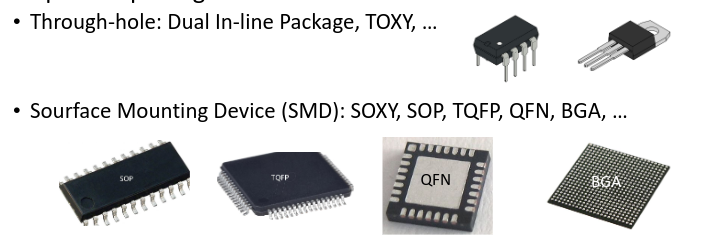
\includegraphics[width=0.5\textwidth]{img/hardware/pcp components.png}
    \caption{Some components of a PCB}
  \end{figure}
\end{section}
\\

A PCB can present different structures, like the one in figure \ref{fig:pcb-structure}. If you take
a look at the double sided one, you can notice that it has two copper layer to which the components
can be connected. Those can be connected in two ways: by vias, which are holes that connect the two
layers, or by traces, which are copper lines that connect the components. The second ones require no
metallization around the holes, being mostly used for mechanical components, whilst the first ones
require a metallization around the holes, being mostly used for electrical components.
\begin{figure}[h]
  \centering
  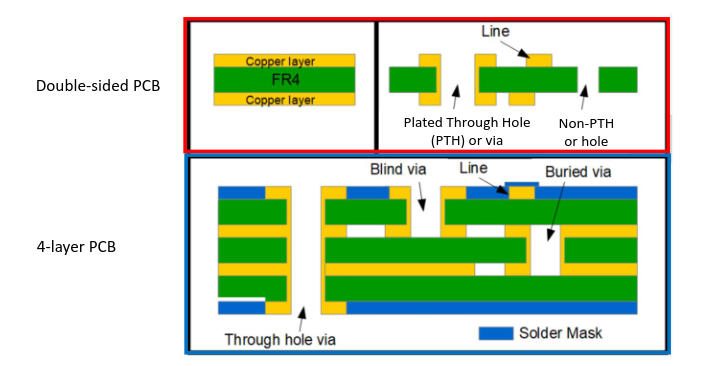
\includegraphics[width=0.7\textwidth]{img/hardware/pcb structure.png}
  \caption{A PCB structure}
  \label{fig:pcb-structure}
\end{figure}
The second example is more complex, being a multi-layer PCB. It has multiple layers, and the
components are connected by vias, which are holes that connect the different layers. The vias can
be of two types: blind vias, which connect the surface layer to the inner layer, and buried vias,
which connect two inner layers. The vias can be filled with a conductive material, like copper, to
improve the connection between the layers.

\begin{section}{Design flow}
  To design a PCB, we must first need to know what to to, and then we can start the design flow by
  using some kind of tools, like Altium Designer, KiCad, or Eagle. The first step is to know exactly
  the footprint of the components, because different components have different footprint, like the
  pin number, the pitch, the size, and so on. This is necessary to know how to place the components
  on the PCB. The second step is to enter the PCB size and design rules in the software, like the 
  minimum trace width. After that, we can start placing the components on the PCB, and then we can 
  start routing them. The last step is to generate the Gerber files, which are the ascii files that
  the manufacturer will use to produce the PCB.
\end{section}

\begin{section}{Security issues}
  Of course, we would like to have a secure board returned by the manufacturer. A trusted supply
  chain is good but not sufficient, in fact one of the biggest issues is to have no leakage of
  information from the integrated circuit, to avoid reverse engineering. At this day, most of PCB
  design have no protection, meaning that any user can try to probe and tamper the board.\\ 
  A board use standard communication protocols, to internal or external communications, and those
  increase the interruptibility of the board, and those can be exploited to extract informations.

\end{section}
